
\begin{center}
   {\colorbox{grey2}{
         \begin{minipage}[t]{0.9\textwidth}
\subsubsection*{Scope}
This Pirana Quick Guide aims to provide an overview of current reporting functionality
available in Pirana.
          \end{minipage}
      }
   }
\end{center}


\subsubsection*{Overview of functionality}
The following functionality for reporting is available in Pirana:
\begin{itemize}
\item Run reports in various formats (HTML, Word, text, LaTeX, 
 pdfLaTeX)
\item Run records of multiple runs (CSV/Excel, HTML, Word, text)
\item Visual interactive run records.
\item Execution log files of executed runs.
\end{itemize}



\subsubsection*{Generating run reports}
\begin{itemize}
\item From the menu or context menu, the option Reports can be accessed, which allows generation of various run reports (Figure \ref{fig:Fig4}) of one or more runs (if more runs are selected simultaneously).
\item The components to be included in the report can be modified (Reports menu, option "Include in reports")
\item Generated run reports are placed into a pirana\_reports folder, and can be accessed from the tab Reports in the right panel of Pirana (Figure \ref{fig:Fig5}). 
\end{itemize}

\begin{figure}[h] \centering
    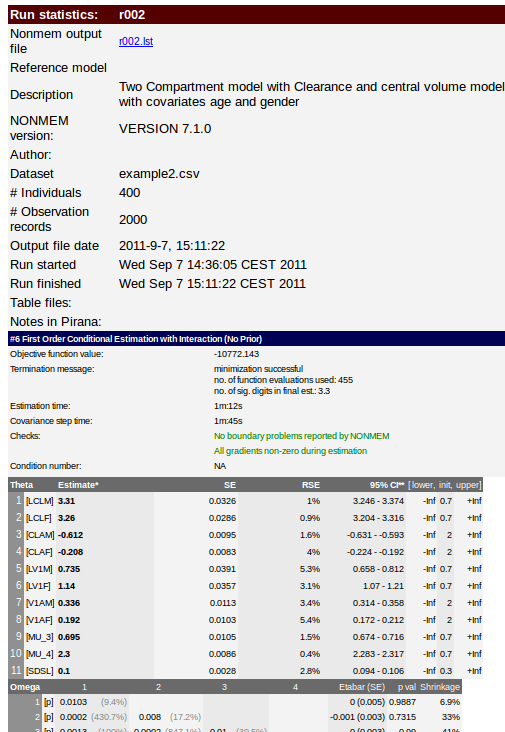
\includegraphics[scale=.4]{images/report_5.png}
    \caption{HTML report\label{fig:Fig4}}
\end{figure}

\begin{figure}[h] \centering
    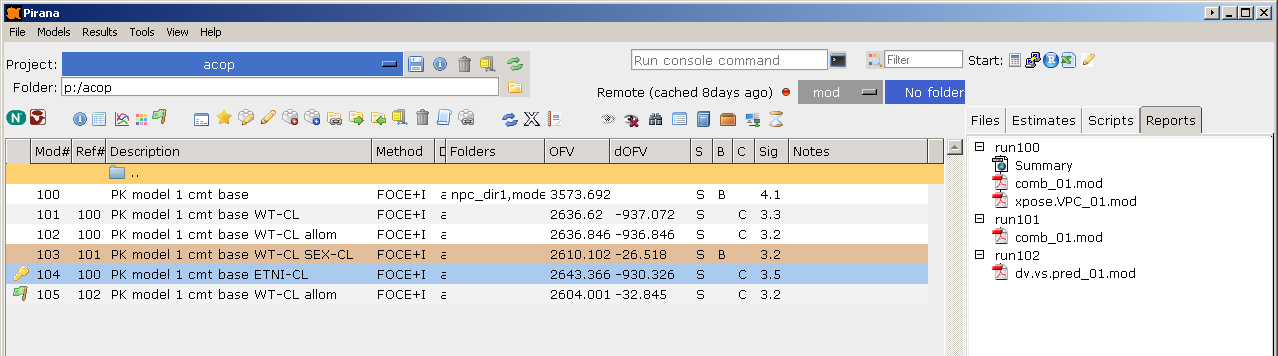
\includegraphics[scale=.25]{images/report_3.png}
    \caption{Overview of available reports in right panel\label{fig:Fig5}}
\end{figure}

\subsubsection*{Generating run records}
\begin{itemize}
\item Run records are documents that contain reports (e.g. as above) for all runs in the project folder.
\item Run records can be created under Results $\rightarrow$ Run records. 
\item The CSV run record is a CSV file that can be opened in excel containing a table of all results (e.g. description, OFV, estimates, RSEs etc) for each model. 
\end{itemize}


\subsubsection*{Generating a visual run record}
\begin{itemize}
\item The visual run record (VRR) is a SVG file which contains an
 interactive tree view of the model development process (Figure \ref{fig:Fig6}. 
\item Models are related to each other based on Pirana's reference model
 tags in the model file.
\item The visual run record can be created under Results $\rightarrow$. 
\end{itemize}

\begin{figure}[h] \centering
    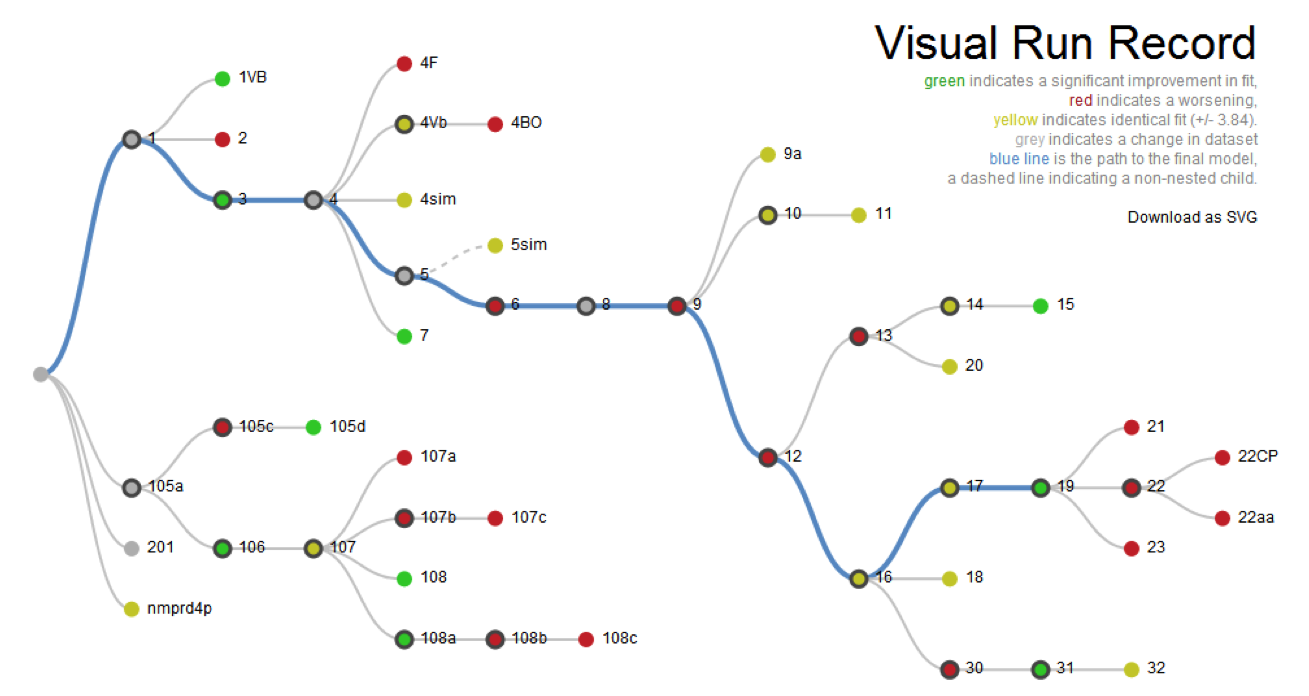
\includegraphics[scale=.4]{images/vrr.png}
    \caption{Visual run record\label{fig:Fig6}}
\end{figure}



